\subsection{Architektur}
Als grundlegende Architektur der Applikation wird das Model-View-Controller (MVC) Konzept verwendet. Controller (in diesem Projekt \emph{Pages} genannt) können zudem Middleware-Komponenten einbinden, welche Funktionalität wie Authentifikation von Requests vor dem Rendering durchführen können.

\vspace{2mm}
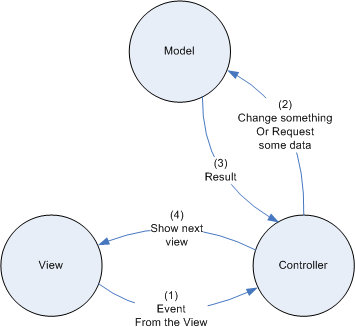
\includegraphics[scale=0.5]{mvcconcept}
\vspace{2mm}

Das Projekt verwendet zudem Singleton-Klassen, um zentrale Funktionalität zu bündeln. Diese werden in sogenannten \emph{Engines} implementiert. Dazu gehören unter anderem Datenbank, Session und Routing.

Es wurde entschieden, ein Index-Rewrite auf dem Webserver zu konfigurieren, um einfachere Pfade verwenden zu können (z.B. \textit{/login} statt \textit{index.php?page=login}) Das Auflösen des Pfades und die Entscheidung, welche MVC Komponenten verwendet werden sollen, übernimmt eine Komponente des \href{https://github.com/steampixel/simplePHPRouter}{steampixel/simplePHPRouter} Frameworks.
